\documentclass[a4paper,11pt]{article}
\usepackage[cm]{fullpage2}
\usepackage{propsections}
\usepackage{graphicx}

\newcounter{note}
\newcommand{\note}[1]{\textbf{NOTE \thenote\addtocounter{note}1: #1}}


\iffalse
   $Id: CaseForSupport.tex 94 2011-02-22 08:13:17Z ucacdxa $
\fi


\begin{document}

\bibliographystyle{unsrt}

\title{Event-based models of disease progression}

\author{Daniel C.\ Alexander (UCL-CS),\\Sebastien Ourselin (UCL-Med.\ Phys.),\\Nick Fox (UCL ION)}

\date{}

\maketitle

\begin{verbatim}
$Id: CaseForSupport.tex 94 2011-02-22 08:13:17Z ucacdxa $
\end{verbatim}

\clearpage


\setcounter{page}{1}

\textbf{PART 1 : TRACK RECORD}\\

\subsubsection*{University College London}
(UCL: \verb+www.ucl.ac.uk+) is ranked fourth in the world and second
in the UK in the 2009 THE-QS universities ranking. The Thomson
Scientific Citation Index shows UCL as the second most highly cited
European university (14th in the world), and as the most cited UK
university by health researchers.

\subsubsection*{UCL's Department of Computer Science}
(UCL-CS: \verb+www.cs.ucl.ac.uk+) is one of the top-ranked computer
science departments both nationally and internationally ($35\%$ of
staff received 4* and $45\%$ received 3* in the last RAE). The
department emphasises experimental computer science and has particular
strengths in computer vision and medical imaging, computer graphics,
machine learning, computer networking, software engineering, human
computer interaction, bioinformatics and information security. We run
advanced master's courses in each of these areas, which provide a
diverse and high quality set of technical lecture courses available to
all researchers at UCL. The PI is in the Vision and Imaging
Sciences (VIS) group (\verb+vis.cs.ucl.ac.uk+).

\subsubsection*{The Centre for Medical Image Computing} (CMIC:
\verb+cmic.cs.ucl.ac.uk+), directed by Prof. Dave Hawkes, formed
in 2005 to bring together technical imaging researchers in UCL-CS and
medical physics with front-line users in medicine and the life
sciences. The centre plays a key role in translating to biomedical
sciences the new developments in imaging methodology arising in
mathematics, computer science, physics, chemistry and the engineering
disciplines. The centre includes five core academic staff (Alexander,
Arridge, Atkinson, Hawkes, Ourselin), over 60 research staff and
students and a diverse group of collaborators including
mathematicians, physicists, life scientists, medical researchers and
clinicians.  Strong links with the Centre for Advanced Biomedical
Imaging (CABI: \verb+www.ucl.ac.uk/cabi+) and several clinical imaging
groups at UCL Hospitals, including the Institute of Neurology (ION),
the Institute of Child Health and the Wellcome Trust Centre for
Neuroimaging, all provide good sources of preclinical and clinical
imaging resources and data, as well as willing volunteers for user
trials of new software, imaging and analysis techniques.

\subsubsection*{The Dementia Research Centre} (DRC: \verb+dementia.ion.ucl.ac.uk+)

The Dementia Research Centre (DRC) at UCL Institute of Neurology has
an international reputation in the study of degenerative dementias.
The Centre is closely integrated with the specialist cognitive
disorders clinic at the National Hospital for Neurology and
Neurosurgery. The DRC has contributed to a number of important genetic
discoveries including finding the first gene for Alzheimer's disease
(AD). Through this work the Centre has established some of the largest
and most important longitudinal studies into familial dementias
including unique cohorts of individuals at risk for familial AD and
other dementias and is the only UK member of the international
initiative on familial AD (the NIH funded DIAN - Dominantly Inherited
Alzheimer Network). The Centre has a particular focus on the use of
imaging and other biomarkers to improve diagnosis in the dementias and
to contribute to finding disease-modifying therapies for these
disorders.

\subsubsection*{The Applicants} are uniquely well placed to carry out
the program of research.  They combine expertise in computational
modelling and parameter estimation (DA), image analysis tools
specifically for neuroimaging (SO), clinical domain knowledge (NF) and
open-source software development (DA, SO).  They have a successful
track record of working together: SO is employed $50\%$ by the DRC,
which provides the front-line application framework for his image
analysis and software development; DA is named collaborator on several
ION program grants and sits on the imaging advisory panel for the DRC.
The preliminary work this project builds on~\cite{FonteijnScience11}
arose from discussions at those panel meetings.  We employed a
post-doc (Hubert Fonteijn) for one year on CMIC's EPSRC platform grant
EP/D506468/01 to initiate the work.  That grant is now finished and
Hubert has taken a job in the Netherlands, but we are eager to develop
and exploit the powerful new ideas that are emerging.

\emph{Prof.\ Daniel Alexander} (DA) has a background in mathematics
and computer science with core expertise in computational modelling
for biomedical imaging.  His PhD work was in computer vision;
specifically, building models of colour image data for autonomous
vehicle guidance~\cite{AlexanderIJCV01}. His emphasis subsequently
switched to medical imaging, although he retains interest in basic
computer vision, eg~\cite{SenanayakeBMVC07}. He is particularly well
known for his work in diffusion MRI where he has developed models at a
range of scales, from microscopic models of fibre
configurations~\cite{JansonsIP03,SeunarineBehrensBook09} and white
matter composition~\cite{AlexanderNI10,ZhangMICCAI10}, to regional
models of parameter trends at the centimetre
scale~\cite{MorganCDMRI10}, up to whole-image models of brain
connectivity~\cite{SherbondyMICCAI10}.  He has developed both simple
parametric models for parameter
estimation~\cite{JansonsIP03,AlexanderNI10} and complex numerical
models for realistic simulation and performance
evaluation~\cite{HallTMI09,PanagiotakiMICCAI10}.  His model-based
approach has led to a variety of significant innovations in diffusion
MRI including acquisition
optimization~\cite{AlexanderNI05,AlexanderMRM08}, pulse sequence
design~\cite{DrobnjakJMR10}, and applications in tractography and
connectivity
mapping~\cite{ParkerPTRS05}, basic
neuroscience and
neuroanatomy~\cite{JonesNI02,ParkerNI05,DraganskiJNeurosci08}, and
various brain diseases~\cite{NewtonBrain06,YogarajahBrain10}.  He has
also worked on model-based approaches in other imaging modalities,
such as magnetization transfer MRI~\cite{CercignaniMRM06} and Computed
Tomography~\cite{PrevostISBI10}.  DA leads development and maintenance
of the open-source Camino (\verb+www.camino.org.uk+) diffusion MRI
toolkit.  The toolkit is popular with users around the globe and the
active mailing list has around 200 recipients.  Camino is a key
vehicle for dissemination of his group's new technical developments in
the area.

DA is an EPSRC Leadership Fellow, since 2008.  The fellowship project
EP/E07748 expands earlier EPSRC projects GR/T22858/01, EP/E056938/1
and GR/R13715/01 on modelling for diffusion MRI modelling to a broader
remit.  DA is also co-founder and steering committee member of the
CONNECT consortium (\verb+www.brain-connect.eu+), which has EU support
and provides complimentary funding for translation of the technology
into neuroscience and medicine.  DA leads the Microstructure Imaging
Group (MIG: \verb+cmic.cs.ucl.ac.uk/mig+), which currently contains 6
PhD students (2 joint with UCL ION; 1 joint with Med. Phys.; 1 joint
with CABI) and 4 post-doctoral researchers (1 joint with CABI).  DA
has graduated 8 doctoral students (no dropouts or failures) since
starting his academic career in 2000.  He has over 160 peer-reviewed
publications. He is reviewer for all the top medical imaging journals
and conferences as well as a wide range of neuroscience, medical and
general science journals and funding bodies around the world. He is
associate editor of IEEE Trans.\ on Medical Imaging (TMI), editorial
board member for NeuroImage, and was program chair of the British
Machine Vision Conference in 2009.

\emph{Dr.\ Sebastien Ourselin} (SO) is Deputy Director of CMIC and
Reader in Medical Image Computing with a strong track record in
biomedical image analysis, clinical software transfer, and research
project management.  He specializes in software development for
collaborative research involving clinical and commercial partners.  SO
has particular expertise in registration and segmentation for
neuroimaging applications.  Has leads development of an open-source
non-linear image-registration package~\cite{ModatCMPB10} with over 500
downloads from \verb+sourceforge.net/projects/niftyreg/+ and now in
commercial development.  That package underpinned the preliminary
work~\cite{FonteijnScience11} for this project.  NiftyReg now forms
part of the NifTK translational imaging software platform
\verb+cmic.cs.ucl.ac.uk/software/+, which also contains software for
cortical thickness measurement, brain segmentation, image
reconstruction and visualization.  NifTK development has direct
support from a CBRC NIHR grant (4/10--3/14; $\pounds545$K).  Initial
focus is on image registration, analysis of cortical thickness, and
pipelining of tools for clinical drug trials; the test version already
has 30-40 users.  Since his re-location to the UK in 2007, SO has
built up a group of 12 researchers developing software for image
registration, segmentation, molecular imaging, statistical shape
modelling, surgical simulation, and image-guided therapy and surgery.
He has published over 140 journal and conference articles. He is
associate editor of Medical Image Analysis and IEEE TMI, and Executive
Secretary of the MICCAI Society. He has chaired or co-chaired several
conferences (DICTA 2003, DICTA 2005, MICCAI 2007).

\emph{Prof.\ Nick Fox MD, FRCP, FMedSci} is a consultant neurologist
and Professor of Clinical Neurology at UCL and a visiting Professor at
the Vrije University, Amsterdam. He holds a Senior Clinical Fellowship
from the MRC and a Senior Investigator Award from the National
Institute of Health Research.  He was recently elected a Fellow of the
Academy of Medical Sciences. He is the only non-US member of the
Alzheimer's Disease Neuroimaging Initiative (ADNI), which is
the largest imaging study of AD. His research has concentrated on
methods, including imaging, for improving diagnosis and assessing
therapies for AD and related disorders.  Image analysis methods that
he helped to develop are now in widespread use in multi-centre
therapeutic trials and academic studies.  He Co-chairs the Research
Advisory Council of the Alzheimer's Society and is a member of the
Scientific Advisory Board of Alzheimer's Research UK.


\subsubsection*{Other collaborators}

include the following:

- Support from the UCL component of the TrackHD initiative; Prof.\
Sarah Tabrizi, who leads medical research team focused on HD.

- Support from the ADNI consortium and access to their data.

- Legion for large data set preprocessing?

\clearpage

\textbf{PART 2 : CASE FOR SUPPORT}

This project establishes a new paradigm for studying the progression
of diseases or developmental processes.  The program of work builds on
our recent innovation~\cite{FonteijnScience11}: the event-based model
of disease progression.  The model provides a temporal signature, the
``progressome'', of the process.  Disease progressomes provide
fundamental new understanding of the disease and offer improved
diagnostic and prognostic accuracy.  The event-based model represents
a new class of computational model that characterizes processes at the
level of a whole cohort or population.  This new way of thinking about
modelling developmental processes reveals a variety of related models
that expose new and different features of the progressome.  This
project first consolidates the original model of this type, the
event-based model, by carefully evaluating and characterizing its
performance both in simulation and then using large real-world
multi-modal data sets.  This leads to both a robust software tool for
wider uptake and new detailed progressomes for two important diseases.
Second, we begin to explore the wider space of related models by
implementing, testing and demonstrating several useful examples.

The project concentrates on disease progression and, specifically,
progression of neurodegenerative diseases.  The ideas all extend to
any kind of disease or more broadly to developmental processes in
general.  However, the aim here is to focus technological development
within a specific application area where we have expertise and unique
access to appropriate data sets.

The specific aims are:

\begin{itemize}

  \item To establish event-based models as a standard tool for disease
progression analysis.

  \item To construct the first multi-modal progressomes for
Alzheimer's disease (AD) and Huntington's disease (HD).

  \item To implement and test new models that capture explicit disease
stages, disease subtypes and causal relationships within the
progressome.

  \item To run the first exploratory analyses of subtypes and causal
relationships in AD and HD.

\end{itemize}

\subsection*{Background}

Modelling patterns of disease progression is a key aim of medical
science. Such patterns provide basic understanding of the disease and
help construct staging systems that assist diagnosis and
treatment.

Disease progression occurs at various levels, ranging from the
symptoms a patient experiences to cellular and biochemical
changes. For example, the first symptom of AD is often a loss of
episodic memory. Progressive deterioration of other cognitive
abilities, such as language and executive function, follows. However,
cellular pathology precedes these symptoms often by many years~\cite{DickersonCerCort09,ScahillPNAS02,ThompsonCerCort01,ThompsonJNeurosci03}. This cellular pathology includes deposition of the protein
beta-amyloid, which forms plaques in the grey matter, and
neurofibrillary tangles (NFTs) within neurons.  Neuronal atrophy
(reduced grey matter volume) also occurs as neurons die.  Cellular
pathology and neuronal atrophy occur earlier in some brain regions
than others and are strongly linked~\cite{HerrupJNeurosci10}, although causal relationships
are yet to be established. Atrophy is easier to observe, because it is
visible in non-invasive imaging techniques like MRI.  The progression
of NFTs and atrophy has a consistent pattern, usually starting in
memory-related areas such as the hippocampus and the entorhinal
cortex, progressing to other higher cognitive areas and finally the
primary cortices~\cite{BraakActaNeuro91}.  All neurodegenerative diseases show some
pattern of atrophy.  However, the progression patterns of other
neurodegenerative diseases are often very different to AD, so the
progression is emerging as a key discriminator of dementias and other
neurodegenerative diseases, which are often confused in clinical
examinations.

Recent efforts of the international medical research community collect
large scale data sets combining clinical, imaging and pathology
measurements from hundreds of patients.  For example, the ADNI
(Alzheimer's Disease Neuroimaging Initiative) consortium has collected
data, including MRI and FDG-PET imaging data, CSF lumbar puncture,
cognitive test results and limited genetic data, from around 700
patients from different centres around the
world~\cite{MuellerAlzDement05}.  The TrackHD initiative is a similar
effort for Huntington's disease~\cite{TabriziLancetNeurol09}.

Despite the availability of this data, current models of disease
progression,
e.g.~\cite{DickersonCerCort09,ScahillPNAS02,ThompsonCerCort01,ThompsonJNeurosci03,JackLancetNeurol10},
remain crude. These models use symptomatic staging to divide the
patients into a small number of groups, such as ``presymptomatic'',
``mild'', ``moderate'' or ``severe''. They then assess the differences
in measurements of pathology among those groups. However, symptomatic
staging relies on imprecise clinical data, and therefore has limited
temporal resolution, which limits the power of the model to
discriminate and stage diseases. The need therefore is urgent for
techniques that exploit large-scale heterogeneous data sets to obtain
detailed models of disease progression that we might truly call a
progressome. Such models will enhance early diagnosis and allow much
more precise staging of patients and thus improve the design and
efficacy of patient-specific treatment plans and drug trials.

The event-based model~\cite{FonteijnScience11} provides a direct
computational approach to modelling disease progression. The model
describes the disease as a sequence of discrete events. The most
closely related models, although somewhat different in formulation,
can be found in paleontology~\cite{PuolamakiPLoSCompBiol06} where
researchers fit timelines of the emergence and extinction of species
to the fossil occurrence of species in different geological time
periods. In disease modelling, the events are changes in patient
state, such as the onset of a new symptom (``patient reports memory
loss to GP'') or the first measurement of tissue pathology (``lumbar
puncture shows raised beta amyloid'', ``hippocampus shows significant
atrophy''). The computational aim is to find the ordering of the
events that is most consistent with a set of measurements from a
cohort of patients. Thus the event-based model provides a semantic
description of the disease similar to a clinician's intuitive
description of its progression.

The input data can be entirely cross-sectional, ie containing a single
snapshot from each patient: at the time of a single examination of
the patient at which measurements are acquired, some events have
occurred while others have not.  So long as the patient cohort
contains sufficient diversity in the advancement of the disease,
snapshots from the whole cohort contain sufficient information to
infer the characteristic pattern.  Longitudinal data, which contains
multiple snapshots from each patient, can provide more robust
information about the progression pattern.  The model adapts naturally
to exploit longitudinal data or, as in~\cite{FonteijnScience11},
heterogeneous data with a mixture of cross-sectional and longitudinal
data.

\begin{figure}
\centering
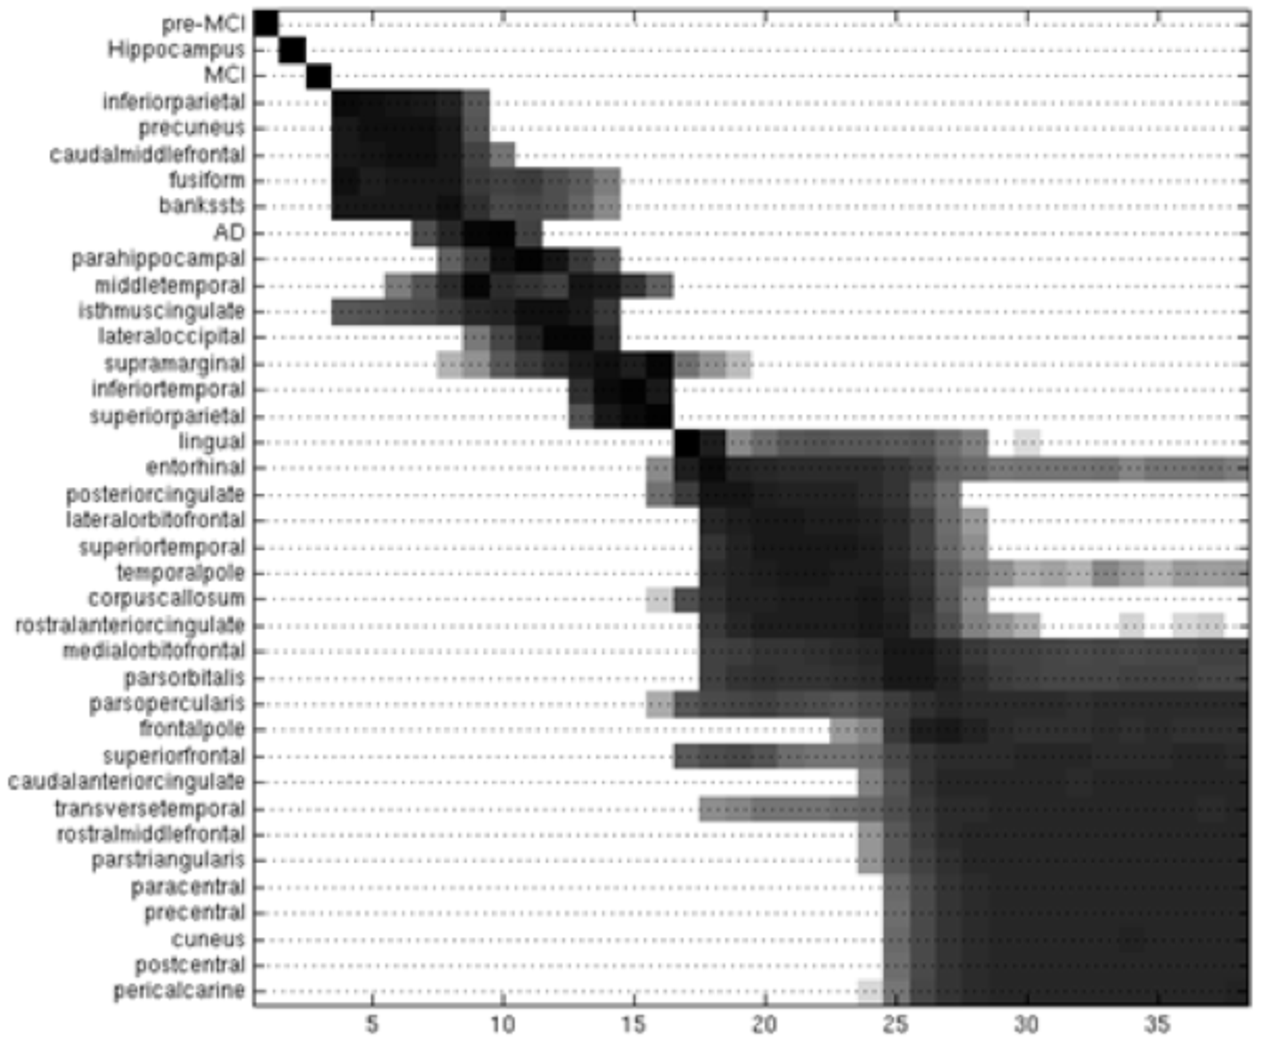
\includegraphics[clip, width=120mm]{fAD_Progressome}
\caption{Preliminary familial Alzheimer's disease progressome from~\cite{FonteijnScience11}.}
\label{fig:progressome}
\end{figure}

To fit the model, we construct a complete forward model that predicts
a set of measurements we obtain from each patient from a candidate
event ordering.  The set of measurements acquired in each exam must
contain at least one measurement sensitive to each event, although the
precise set may vary from patient to patient and the formulation is
robust to missing data.  The forward model provides a mechanism to
evaluate the likelihood of the data set given a particular event
ordering and thus to sample the posterior distribution on the ordering
given the data using, for example, Markov Chain Monte Carlo (MCMC).
Figure~\ref{fig:progressome} shows an example progressome obtained in
this way from an imaging data set acquired from a familial AD cohort.
In the figure, the events are the emergence of atrophy in different
regions of the brain.  Each patient snapshot comes from a pair of
conventional T1-weighted MRIs at least 12 months apart.  The
FreeSurfer software~\cite{FischlNeuron02} identifies around 30 separate
anatomical regions in the baseline image.  Non-linear
registration~\cite{ModatCMPB10} warps the later image to align with the
baseline and thus provides measurements of volume change in each
FreeSurfer region.  We evaluate the likelihood of atrophy by
comparison with a similar set of measurements taken from control
subjects.  The order of the events along the vertical axis in
figure~\ref{fig:progressome} is the most likely ordering given the
atrophy measurements (MCMC sample with highest likelihood).  Each row
shows the posterior distribution on the order position for the
corresponding event, ie the histogram of positions over a large number
of MCMC samples.

The progressome reveals not only the most likely ordering of events,
but also gives unique insight to the variability of the progression
pattern, which no previous models
provide. Figure~\ref{fig:progressome} shows clearly that the
separation of consecutive events is often weak, suggesting that they
frequently interchange between patients or occur
simultaneously. However, events further apart in the ordering show no
overlap in positional variance, demonstrating that their temporal
separation is consistent over the cohort and a strong feature of the
disease progressome. Moreover, consecutive clusters of regions often
emerge, where ordering within the clusters is weak (extensive overlap
of region positions within the cluster), but ordering between clusters
is strong (little or no overlap of the clusters). These clusters
suggest separations into groups of events that may define useful
disease stages.  Further experiments in~\cite{FonteijnScience11}
demonstrate use of the model for staging new patients: given unseen
data, we can determine the most likely position of that patient where
preceding events have occurred, but later events have not.

The preliminary work in~\cite{FonteijnScience11} tests the event-based
model on two small data sets.  The first is the familial AD data set
from~\cite{RidhaRad07}.  The cohort contains only 9 patients, although
the number of separate visits varies from 3 to 8 (total of 41 scans),
and 25 controls with 2 scans each.  Despite the sparse sampling, the
event-ordering algorithm confirms the broad pattern of disease
progression earlier work~\cite{BraakActaNeuro91,ScahillPNAS02}
suggests, but new detail, such as the relatively late appearance of
significant atrophy in the entorhinal cortex.  The second data set is
the London HD data set~\cite{HenleyJNeurol09}.  Results show very
different orderings and patterns to the fAD cohort with clear contrast
between the progressomes of these two neurodegenerative diseases.

In summary, early results from the basic event-based model are very
promising and already provide new insight in two important diseases.
However, work is still required to establish the technique and enable
it to produce results that medical researchers and clinicians will
trust.  Moreover, the data sets we have used so far are insufficient
to determine a complete progressome of either disease, because (i) the
number of patients is small, (ii) they contain only MRI data and a
small amount of clinical information, and (iii), particularly for HD,
they do not cover the full range of disease stages.  Thus, in WP1,
this project performs the necessary evaluation to characterize and
maximize the performance of the model, and understand the results
allowing researchers to draw solid and informed interpretations and
conclusions.  WP2 then constructs the first progressomes from two
large-scale data sets.  Finally, WP3 explores a variety of related but
new models to establish efficacy of estimating various new features of
disease progressomes.

\subsection*{Programme and methodology}

The program of work divides into three work packages.

\subsubsection*{Work Package 1: Validation and software (low risk, medium
impact)}

This work package consolidates the basic event-based model with
evaluation and validation experiments and delivers a self-contained
software package to allow widespread application of the technique.

Task 1.1. M1-2. Develop a simulation package and evaluate performance
statistics as a function of data size and quality.

Task 1.2. M3-6. Evaluate performance as a function of preprocessing
options to optimize the preprocessing pipeline.  For imaging
applications, such as those in~\cite{FonteijnScience11} and WP2, image
preprocessing steps, such as segmentation and registration, are
critical for reliable measurements of atrophy.  We will assess various
segmentation and registration combinations for measurement of atrophy
by comparison with manual segmentations on a small subset of images.
We will further assess different measures of brain atrophy, such as
volume change or cortical thickness, to determine those most reliable
for constructing progressomes in neurodegenerative disease.

Task 1.2. M6-7. Quantify the ability of the fitting algorithm to
identify misclassified data sets.  A complication with ADNI in
contrast to the familial AD data set we have used previously is that
diagnosis is unconfirmed in sporadic AD until after death.  Familial
AD is genetically determined so we can guarantee that all patients in
the cohort are correctly diagnosed.  The misdiagnosis rate of AD is
around $5\%$ and we need to determine how this level of corruption
effects the fitted progressome.

Task 1.3. M8. Write up and publish the optimized pipeline and
performance statistics in a technical journal.

Task 1.4. M9. Publish event-based model code on the Internet with
detailed documentation, user manual and guidance.

Task 1.5. M10-30. Extend simulation package for new models.

Task 1.6. M24-36. Add new models to release code when ready.

\subsubsection*{Work Package 2: Large data sets (medium risk, high
impact)}

This work package runs the basic event-based model on two large
multi-modal data sets to generate comprehensive progressomes for AD
and HD.  Specifically, we will use the ADNI and TrackHD data sets to
construct detailed progressomes for each disease.  The progressomes
will add fundamental new knowledge about each disease.  More broadly,
they provide demonstrators of the tools developed in this project to
facilitate uptake by other researchers with similar data sets in other
applications.

Task 2.1. M7-8. Preprocess ADNI and TrackHD data sets.

Task 2.2. M7. Extend the event-based model code to handle additional
data types.  In particular, CSF from lumbar puncture, cognitive and
amyloid deposition from FDG-PET, as well as MRI.

Task 2.3. M9-11. Estimate the AD and HD progressomes.

Task 2.4. M12. Publish high impact clinical papers presenting the
first progressomes.

\subsubsection*{Work Package 3: Alternative models (high risk, high impact)}

This work package develops various new models that extend the basic
event-based model in~\cite{FonteijnScience11} to reveal new features
of the progressome.  The models all fit in the broad class of
event-based models, but use more complex data structures than the
strict linear ordering in the original model to express different
relationships between events.  Specifically, we will study four new
kinds of model:

\begin{itemize}

\item \emph{Ordered-groups models} provide an optimal stratification
of disease stages.  The model assigns each event to one of a set of
groups.  Each group represents the disease stage during which all the
events in that group occur.  The groups have a strict ordering, but
the order of all events within each group is undetermined.  Further
extensions might represent the ordering using pq-trees or other
hierarchical data structures to allow partial orderings or some events
to have less well defined position than others.

\item \emph{Absolute time} is purposefully factored out in the
event-based model to focus on the order of events independently of
different rates of degeneration among the patient cohort.  However,
the rate of degeneration can be an important factor discriminating
diseases and subtypes.  We can bring absolute timings back into the
progressome by adding extra model parameters that capture times
between pairs or groups of events.

\item \emph{Mixture models} combine multiple progressomes on the
assumption that the cohort contains subtypes of patients with
different disease variants that have distinct progression patterns.
Alzheimer's is known to have subtypes with different progression
pattern, such as visual variant AD in which atrophy occurs in
the vision regions of the brain earlier than the main phenotype.

The basic event-based model is robust to the presence of subtypes with
distinct progression patterns even though it does not capture them
explicitly.  Groups of events that exhibit different trajectories
among subtypes simply appear weakly ordered in a single event-based
model like the blocks in figure~\ref{fig:progressome}.  However,
explicitly modelling the subtypes can provide greater detail for each
subtype.

Further refinement might allow the orderings of each subtype to
overlap.  For example, the event ordering for subtypes may differ only
in a small subset of the events.  Our Bayesian estimation framework
facilitates model selection to identify the most parsimonious
description of the data through mixtures of partially overlapping
event orderings.

\item \emph{Causal models} reveal candidate causal relationships
between events comprising the progressome.  Covariance of the timings
of two events suggests a causal relationship between the two events.
Causality may not be direct, as covariance may arise if both events
are consequences of some third event even if they do not interact with
one another directly.  However, the model at least reveals candidate
causal links, which intervention experiments might subsequently test.

\end{itemize}

The Bayesian formulation we have developed for the event-based model
extends naturally to allow fitting all the alternative models above.
It enables two distinct modes of operation: hypothesis testing and
exploratory.  In hypothesis testing, eg the existence of two subtypes
or a causal link between two events, we compare models with and
without the subtypes or causal link and determine which model
maximizes the likelihood of the data.  In exploratory analyses, we fit
a larger range of models, eg with $1,\cdots,N$ subtypes or all
permutations of causal links between event pairs.  The Bayesian
formulation provides the likelihood of the data for each candidate
model; the model that maximizes the likelihood suggests a set of
subtypes or causal relationships.

Task 3.1. M13-16. Implement and test the groups model.  Extend the
simulation framework to allow basic evaluation.  Evaluate the
performance and behaviour of the model as a function of data
properties.  Publish a technical methods paper.

Task 3.2. M17-18. Generate group-based progressomes from ADNI and TrackHD data
sets.  Publish high-impact clinical papers.

Task 3.3. M13-20. Augment event-based models with absolute time parameters.
Test and evaluate in simulation.  Produce augmented progressomes with
new models.

Task 3.4. M21-26. Implement subtype models.  Test and evaluate in
simulation and using known mixtures, such as half-AD-half-HD data
sets.  Test on fronto-temporal dementia (FTD) cohort data available
from DRC (FTD has genetically determined subtypes).

Task 3.5. M27. Run exploratory analyses on ADNI and TrackHD data sets to
determine the set of subtypes each data set supports.

Task 3.6. M28-33. Implement and test causal models in simulation.

Task 3.7. M34. Run exploratory analyses for causal relationships in ADNI
and TrackHD.

Task 3.8. M35-36.  Write up.

\clearpage
\bibliography{Progression}


\clearpage


\note{These are the JeS form sections.}

\section*{Objectives}

\begin{itemize}

\item To evaluate and characterize event-based models of disease
progression.

\item To release open-source software for event-based model estimation.

\item To construct a multi-modal event-based model for
Alzheimer's disease from the ADNI data set.

\item To construct a multi-modal event-based model for
Huntington's disease from the TrackHD data set.

\item To establish efficacy of variants of the basic event-based model
including staging models, subtype models and causal models.

\end{itemize}


\section*{Summary}

The project develops new computer modelling technology for determining
the progression pattern of diseases.  The temporal evolution, or
progressome, of a disease is a fundamental characteristic that
distinguishes it from other diseases.  However, a detailed description
of a disease progressome is difficult to obtain even from rich
longitudinal data sets, because disease progression can vary
substantially between individuals.  The event-based modelling approach
we develop here provides a natural framework for describing diseases,
and developmental processes in general, in terms of the sequence of
events that occur and the variability of the order of events over the
population.  It fuses information from diverse sources, such as
imaging data, cognitive tests, clinical exams and blood tests, to
obtain a uniquely rich description that will enable earlier and more
accurate diagnosis and more precise staging improving personalized
treatment and care plans.

We have recently published a preliminary study using the event-based
model, which provides very promising results.  This project performs
the necessary refinement and evaluation to establish the new technique
as a widespread tool for progression analysis and as a working
diagnostic aid.  We demonstrate the technique by using it to create
the first detailed progressomes of both Alzheimer's disease and
Huntington's disease.  Both are fundamental advances in medical
science in their own right, although their role in this project is
also to serve as demonstrators to facilitate broader uptake of the
ideas in a wider range of applications in the future.

The project also explores a range of new and more sophisticated models
within the same family that potentially reveal a range of new features
of the progressome.  Specifically, we devise new models that
incorporate disease stages, disease subtypes and causal relationships
between the events that comprise the disease.  The new models, in
combination with large data sets that several world-wide initiatives
are currently collecting, have the potential to provide fundamental
new information about diseases that will feed directly into treatment
development and trials.  Here, we perform an initial study of their
feasibility and characterize their performance and potential.

\section*{Academic beneficiaries}

The following academic communities will benefit directly from the
work:

\begin{itemize}

\item Medical researchers and drug developers will benefit from the
new tools providing earlier and better diagnosis.  This identifies
more specific cohorts more precisely, which reduces patient numbers
required for clinical trials and expedites translation of candidate
treatments to market.

\item The broader life sciences community will benefit from having the
new tool available for analysis of progression of any developmental
process.  To give a very simple example in early childhood, the
event-based model might provide a characteristic ordering of the
events ``first tooth'', ``first word'', ``myelination in the corpus
callosum'', ``starting to walk'', ``emergence of visual attention
skills'', ``visual self recognition'' and how that ordering varies
over the population.  Moreover, it can construct the ordering and its
variability from a sparse set of snapshots taken from a cohort
children in a short period of time and does not require longitudinal
monitoring.  The tool becomes particularly powerful when combined with
other phenotypical information: does the progression pattern differ
between preterm and term infants?  Does it differ in disorders like
autism?

\item The project introduces a new area of computational modelling
that provides rich new research opportunities for that community in
exploring the variety of population models capturing different
relationship between events that comprise developmental processes.

\item The image analysis community will benefit since the tools they
develop are essential for using the new techniques we propose here in
imaging applications.

\end{itemize}

\section*{Impact summary}

Management and treatment of neurodegenerative diseases is one of the
biggest challenges facing medicine today.  For example, Alzheimer's
disease is the most common form of dementia, and the US alone has 5
million sufferers.  Their direct medical costs exceed $\$250$ billion
and that figure is rising rapidly with the ageing population.  No
disease-modifying drugs are currently available and the situation is
similar for many other neurodegenerative diseases.  However, research
into possible treatments is intensive and viable options are in the
pipeline.  To bring such treatments to market requires large scale
clinical trials with appropriate patient cohorts.  Lack of early and
accurate diagnosis is a major obstacle to these trials.  The current
gold-standard diagnosis for Alzheimer's disease remains post-mortem
histology and clinical diagnostic accuracy is only around $80\%$,
because the symptoms are easily confused with other dementias and
psychiatric disorders.  The progressomes we establish here fuse
information from multiple independent sources naturally to improve
diagnostic accuracy and patient staging.  They will have a major
impact both in the development of treatments, by identifying
appropriate patient cohorts more precisely, and in designing
personalized treatment plans for patients earlier and better.

The new models we propose for subtyping and causal analysis will have
far-reaching impact in the longer term.  Neurodegenerative diseases
often have several subtypes that may require different treatments or
care plans.  Identifying those subtypes again assists drug trials,
expedites bringing effective treatments to market, and further
pinpoints personalized treatment plans.  Identifying causal links
between events provides new understanding that guides future drug
development, by focusing efforts on root causes rather than emergent
symptoms.


\section*{Suggested revivewers}

\begin{itemize}

\item Michael Wiener, University of California, San Francisco.
Principal investigator of ADNI.

\item Clifford R.\ Jack, Mayo Clinic, Minnesota.  Clinical expertise
in Alzheimer's disease and modelling progression.

\item Daniel Rueckert, Imperial College.  Image analysis and
computational modelling for biomedical imaging.

\end{itemize}


\clearpage
\setcounter{page}{1}

\section*{Pathways to impact}

Impact of the project depends on successful dissemination of the ideas
to the potential beneficiaries, through publications, presentations
and demonstrations, and through appropriate design and distribution of
software tools and documentation to enable straightforward access,
installation and application by potential users.

\subsection*{Knowledge and information dissemination}

The primary mechanisms are:

\begin{enumerate}

\item Technical journal publications to document performance
statistics and data requirements.  These publications will
characterize the capabilities and limitations of the models, specify
precisely how to interpret results and explain what conclusions we can
and cannot draw in different situations.  We will aim for journals
such as IEEE TMI, Medical Image Analysis, and NeuroImage.

\item High-impact journal publications in general science journals,
such as Nature, Science, Proc.\ National Academy of Sciences,
introducing the new models.  The family of models we explore is very
new and has very wide potential application, so publication in general
science journals is feasible and appropriate, to expose the ideas to
as wide an audience as possible..

\item Publications in major clinical journals, such as New England
Journal of Medicine or The Lancet, to expose the key results, such as
the AD and HD progressomes, to a broad medical community likely to
utilize the results directly and to adopt similar methods in other
applications.

\item Technical conference publications and presentations at medical
imaging conferences (MICCAI, ISMRM), machine learning conferences
(ICML) and computational modelling conferences (COSINE) to disseminate
technical ideas to, and get feedback from, the technical community
rapidly during development.

\item Applications conference presentations and demonstrations, at, for
example, HBM and RSNA, to engage with the community likely to use the
ideas in neuroscience and medical applications.

\item Project meetings for example within the CONNECT and ADNI
consortia, and within the UCL Neuroscience community,
\verb+www.ucl.ac.uk/neuroscience+, and medical school provide smaller
scale, but nevertheless valuable and more direct, dissemination.

\end{enumerate}

The work plan includes X man-months explicitly for writing
journal and conference publications.  We include costs for attendance
at Y different conferences to pursue dissemination, although we will
attend additional relevant conferences through other related projects.

\subsection*{Software dissemination}

The primary mechanisms are:

\begin{enumerate}

\item Release a new software package to disseminate the techniques.
  Both DA and SO have a long track record and experience of
  maintaining open-source software.  See Camino
  \verb+www.camino.org.uk+ and the NifTK
  \verb+cmic.cs.ucl.ac.uk/software+.

\item Documentation will include case studies that document the
precise processing steps that produce the key results in the high
impact papers.  These will provide valuable demonstrators to other
potential users enabling them to replicate standard procedures before
tailoring them to their needs rapidly and without waiting for input
from the developers.

\item If appropriate and the demand is sufficient, we will run
educational workshops connected with appropriate conferences to run
specific demonstrations and teach users how to get the best out of the
available tools.

\end{enumerate}

\subsection*{Follow-on funding}

As the project develops and the core techniques become established, we
will seek funding to explore a wider range of applications.  Mostly we
envisage achieving this through studentships joint with appropriate
domain experts and funded by charities or UCL doctoral training
programs.  Here are some specific examples:

\begin{itemize}

\item A nice PhD project would focus on progression analysis of
Alzheimer's disease using the DIAN data set.  DIAN has much richer
genetic information than ADNI, allowing a detailed exploration of the
relationship between genetic profiles and the AD progressome.

\item Childhood development studies in collaboration with ICH.
\note{Ask Chris Clark about possible data sets.}

\item Studies of normal aging using for example the 1946 cohort data
set (a small cohort of post-war baby boomers tracked through life with
medical history, life changing events etc).  A smaller 1936 cohort
also has imaging data.

\item If the early tests of causal analysis in WP3 prove successful,
we can start to test some long standing questions about causal
relationships in AD, such as the amyloid hypothesis (amyloid
deposition causes neuronal loss) and connectivity of loss (atrophy
follows white matter connections).  New data sets currently being
acquired, such as ADNI2, which includes diffusion tensor imaging and
resting state fMRI data that supports connectivity analysis, in
combination with interventional studies, potentially on cohorts of
animal models, and the models we develop here provide a possible
approach to addressing these difficult questions.

\item Other brain diseases such as multiple sclerosis, prion diseases.

\item Non-brain diseases: cancer, AIDS, diabetes, childhood asthma.

\end{itemize}


\subsection*{Engage industry}

Also once the techniques become established, we will be in a position
to work with drug companies to tailor the techniques for use in cohort
selection for clinical trials or for studying differences in
progression patterns for treated and untreated cohorts.  The
applicants have strong links with various pharmaceutical companies.
DA has a CASE studentship supported by GSK.  \note{Check with Nick.}





\clearpage

\section*{Justification of resources}

Prof.\ Alexander will take overall responsibility for managing the project.

\subsubsection*{Personnel}: Two post-docs for three years.

One algorithms person based in computer science with theoretical
expertise in modelling and learning.  This person will develop the
core implementations of all the models and fitting routines, develop
the simulation system and use it for performance evaluation, lead
writing of the modelling and evaluation papers.

One more experienced research, possibly Matt Clarkson, who is
fundamentally a computer scientist but with good understanding of the
applications end.  This researcher will lead evaluation and refinement
of preprocessing steps, run and validate preprocessing of ADNI and
TrackHD data, run the software to generate the final progressomes,
liaise with clinical collaborators to ensure quality of results and
get good interpretations to maximize the impact of the work, lead
writing of high impact clinical papers in collaboration with clinical
partners.

$10\%$ of a technician.

\note{Possibly 1y of a clinical fellow?}

\subsubsection*{Travel}: one national, one international conference
per researcher per year.

\subsubsection*{Equipment}: Decent desktop and laptop for each researcher.
Contribution to COMIC cluster to buy dedicated time when necessary, eg
preprocessing of ADNI and TrackHD data sets.

\subsubsection*{Total}: probably around 750K.








\end{document}

